\section{View Handler}


Das View Handler Design-Pattern hilft alle Views welches ein Softwaresystem bereitstellt zu verwalten. Eine View-Handler Komponente erlaubt es Clients Views zu öffnen, zu verändern und zu entsorgen. Es koordiniert zudem die Abhängigkeiten zwischen Views und kümmert sich um ihre Aktualisierung.

\subsection*{Example}


Ein Multidokument-Editor erlaubt es an mehreren Dokumenten gleichzeitig zu arbeiten. Jedes Dokument wird in seinem eigenen Fenster (Moderner: Tab) angezeigt.

Um solche Editoren effizient zu benutzen benötigen Benutzer hilfe beim Verwalten der Fenster. Zum Beispiel möchten sie ein Fenster klonen um mit mehreren unabhängigen Ansichten auf das selbe Dokument arbeiten zu können. Oft schliessen Benutzer nicht alle Fenster bevor sie die Anwendung beenden. Es ist die Aufgabe des Systems alle offenen Dokumente zu überwachen und sie vorsichtig zu schliessen. Änderungen in einem Fenster können auch andere Fenster betreffen. Deshalb benötigen wir einen effizienten Update-Mechansimus um die Änderungen zwischen Fenstern zu propagieren.

\subsection*{Context}


Ein Software-System stellt verschiedene Views von applikationsspezifischen Daten zur Verfügung order unterstützt das Arbeiten mit mehreren Dokumenten.

\subsection*{Problem}


Software-System welche mehrere Views unterstützen brauchen oft zusätzliche Funktioanlität um die Views zu verwalten. Der Benutzer will bequem Views öffnen, verändern oder entsorgen. Ein Update einer View soll autoamtisch an die entsprechenden anderen Views weitergegeben werden.

\subsubsection*{Forces}


\begin{itemize}
	\item Mehrere Views sollen durch den Benutzer wie auch durch interne Komponenten des Systems einfach verwaltet werden können.
	\item Die Implementierung der Views darf nicht von anderen Views abhängig sein oder mit dem Code gemsicht werden welcher zur Verwaltung der Views dient.
	\item Die Implementierung der Views kann varieren und weitere Arten von Views können während der Lebenszeit des Systems hinzugefügt werden.
\end{itemize}

\subsection*{Solution}


Trenne die Verwaltung von Views vom Code welcher die spezifischen Views repräsentiert oder kontrolliert.

Eine View Handler Komponente verwaltet alle Views welche das Software-System bereitstellt. Es bietet die notwendige Funktionalität an um Views zu öffnen, zu koordinieren und zu schliessen, und zudem um die Views zu bedienen. Zum Beispiel ein Kommando um alle Views in einer gekachelten Ansicht zu arrangieren.

Spezfische Views werden in separaten View-Komponenten gekapselt, zusammen mit der Funktionalität sie darzustellen und zu kontrollieren. Suppliers versorgen die Views mit den Daten welche sie anzeigen sollen.

Das View Handler Pattern adaptiert die Idee die Präsentatiion von der Funktionalität zu trennen, wie beim Model-View-Controller Pattern. Es stellt nicht die Struktur des gesammten Software-Systems zur Verfügung, sondern entfernt jediglich die Verantwortung die Gesamtheit der Views zu verwalten von den Model- und View-Komponenten. Das Pattern überträgt diese Verantwortung an die View Handler Komponente.

Die View Handler Komponente lässt ich auch als Abstract Factory (GOF) oder als Mediator betrachten. Sie ist eine Abstract Factory, da die Clients unabhängig davon sind wie eine spezifische View erstellt wird. Sie ist ein Mediator weil die Clients unabhängig davon sind wie die Views koordiniert sind.

\subsection*{Structure}

\begin{figure}[H]
	\centering
	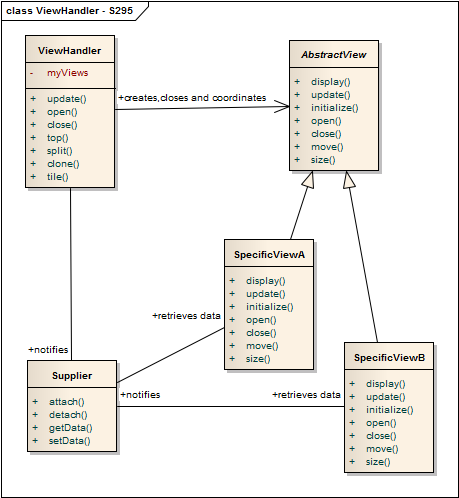
\includegraphics[width=0.7\textwidth]{content/posa1/images/view-handler-classes.png}
	\caption{View Handler Klassendiagramm}
\end{figure}


Der View Handler stellt auch Funktionen bereit um die Views zu schliessen, sowohl einzelne Views als auch alle Views auf einmal.

Die Hauptverantwortung des View Handler ist es jedoch die Views zu verwalten. Zum Beispiel um eine View in den Vordergrund zu holen, alle Views zu kacheln , eine einzelne Views in mehrere Teile zu teilen, alle Views zu aktualisieren und um Views zu klonen.

Eine Abstract View Komponente definiert eine gemeinsame Schnittstelle (Interface) für alle Views. Der View Handler benutzt diese Schnittstelle um die Views zu erzeugen, zu koordinieren und zu schliessen. Die dem System zu grunde liegende Plattform benutzt die Schnittstelle um Benutzerereignisse auszuführen, wie zum Beispiel das vergrössern eines Fensters.

Spezifische View-Komponenten leiten von der Abstract View ab und implementieren die Schnittstelle. Jeder View implementiert seine eigene "display" Funktion. Diese empfängt Daten von Suppliers der View, bereitet diese Daten zur Anzeige vor und präsentiert sie dem Benutzer. Die "display" Funktion wird aufgerufen beim Öffnen oder Aktualsieren der View.

Supplier Komponenten stellen die Daten, welche durch View-Komponenten angezeigt werden, zur Verfügung. Sie stellen eine Schnittstelle zur Verfügung welche es Clients - wie zum Beispiel Views - erlaubt Daten zu empfangen oder zu ändern. Sie benachrichtigen abhängige Komponenten über Änderungen an ihrem internen Zustand. Solche abhängige Komponenten können Views oder falls der View Handler Aktualisierungen durchführt der View Handler selbst sein.

\subsection*{Dynamics}

\begin{figure}[H]
	\centering
	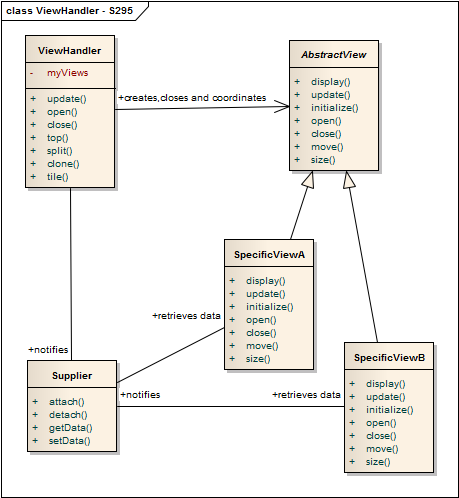
\includegraphics[width=0.7\textwidth]{content/posa1/images/view-handler-classes.png}
	\caption{View Handler Klassendiagramm}
\end{figure}

\subsubsection*{Szenario 1: Ein View Handler erzeugt eine neue View}

\begin{enumerate}
	\item Ein Client weist den View Handler an eine neue View zu öffnen.
	\item Der View Handler instanziert und initialisiert die entsprechende View. Die View registriert sich beim Change-Propagation Mechanismus seines Supplieres, entsprechend dem Publisher-Subscriber Pattern.
	\item Der View Handler fügt die View zur internen Liste von geöffneten View hinzu.
	\item Der View Handler weist die View an sicht selbst anzuzeigen. Die View öffnet ein neues Fenster, empfängt Daten von seinem Supplier, bereitet die Daten zur Anzeige vor und präsentiert sie dem Benutzer.
\end{enumerate}

\subsubsection*{Szenario 2: Ein View Handler kachelt die Views }
\begin{enumerate}
	\item Der User führt das Kommando aus um alle offenen Fenster zu kacheln. Der View Handler empfängt die Aufforderung.
	\item Für jedes offene Fenster berechnet der View Handler eine neue Grösse und Position und ruft die entsprechende Resize und Move Prozeduren auf.
	\item Jede View ändert seine Position und Grösse und stellt die entsprechende Clipping-Fläche ein. Sie aktualisiert das Bild und zeigt es dem Benutzer an. Wir nehmen an, dass die Views die Daten welche sie anzeigen in einem Cache halten. Ist das nicht der Fall müssen die Views die Daten von ihren Supplieren neu beziehen.
\end{enumerate}

\subsection*{Implementation}
\begin{enumerate}
	\item Identifiziere die Views
	\item Spezifiere eine gemeinsame Schnittstelle für die Views
	\item Implementiere die Views.
	\item Definiere einen View Handler. Implementiere die Funktionen um neue Views zu erzeugen als Factory Methods (GOF).
\end{enumerate}


\subsection*{Variants}


View Handler with Command objects. Diese Variante benutzt Command Objects um ViewHandler unabhängiger von der Implementation der Views zu machen. Statt die View-Funktionalität direkt aufzurufen, erstellt der View-Handler ein entsprechendes Command und führt dieses aus. Eine weitere Möglichkeit wäre es, Commands zu erstellen und diese einem Command Prozessor (POSA1, nicht behandelt) zu übergeben. Dies erlaubt zusätzliche Funktionalität wie das Rückgängigmachen eines ausgeführten Commands.

\subsection*{Known Uses}


\begin{itemize}
	\item Macintosh Window Manager
	\item Microsoft Word
\end{itemize}

\subsection*{Consequences}


\subsubsection*{Benefits}


\begin{itemize}
	\item Einheitliches Handhaben der Views (-> gemeinsame Schnittstelle), alle Komponenten können über ein Interface auf die Views zugreifen, unabhängig von deren Inhalt
	\item Erweiterbarkeit und Austauschbarkeit der Views
	\item Applikationsspezifische View-Koordination, da Views von einer zentralen Instanz verwaltet werden, können spezifische Koordinationsstrategien verwendet werden. Koordinationsstrategien können auch benutzt werden, um die Applikation auf verschiedene Displaytypen anzupassen (z.B. kleine Smartphones vs Desktopbildschirm)
\end{itemize}

\subsubsection*{Liablities}


\begin{itemize}
	\item Beschränkte Anwendbarkeit. ViewHandler lohnen sich nur, falls viele unterschiedliche Views, Views mit logischen Abhängigkeiten zwischeneinander oder unterschiedliche Koordinationsstrategien unterstützt werden müssen. Andernfalls erhöht ein View Handler bloss den Implementationsaufwand und die Komplexität der Software.
	\item Effizienz. Da zusätzliche Zwischenschicht. Meist nicht wirklich ausschlaggebend.
\end{itemize}

\subsection*{See also}

\begin{itemize}
	\item Model View Controller
	\item Presentation-Abstraction-Control
\end{itemize}


